% user_manual.tex
% User manual for the 1-D marine particle coagulation column model.


\documentclass[12pt,a4paper]{report}

\usepackage[margin=2.5cm, headheight=15pt]{geometry}
\usepackage{amsmath, amssymb}
\usepackage{graphicx}
\usepackage{booktabs}
\usepackage{longtable}
\usepackage[hidelinks]{hyperref}
\usepackage{listings}
\usepackage{xcolor}
\usepackage{parskip}
\usepackage{microtype}
\usepackage[T1]{fontenc}
\usepackage{lmodern}
\usepackage{fancyhdr}
\usepackage{emptypage}
\usepackage{pdflscape}
\usepackage{titlesec}


% Reduce chapter and section heading sizes
\titleformat{\chapter}[hang]{\large\bfseries}{\thechapter.}{0.6em}{}
\titlespacing*{\chapter}{0pt}{20pt}{10pt}
\titleformat{\section}{\normalsize\bfseries}{\thesection}{0.5em}{}
\titlespacing*{\section}{0pt}{10pt}{4pt}
\titleformat{\subsection}{\normalsize\itshape}{\thesubsection}{0.5em}{}
\titlespacing*{\subsection}{0pt}{8pt}{2pt}

% ---- page style ----
\pagestyle{fancy}
\fancyhf{}
\fancyhead[L]{\nouppercase{\leftmark}}
\fancyhead[R]{}
\fancyfoot[C]{\thepage}
\renewcommand{\headrulewidth}{0.4pt}

% plain style for chapter-opening pages
\fancypagestyle{plain}{%
  \fancyhf{}
  \fancyfoot[C]{\thepage}
  \renewcommand{\headrulewidth}{0pt}
}

% ---- code listing style ----
\lstdefinestyle{matlab}{
    language=Matlab,
    basicstyle=\ttfamily\footnotesize,
    keywordstyle=\color{blue},
    commentstyle=\color{gray},
    stringstyle=\color{teal},
    numbers=left,
    numberstyle=\tiny\color{gray},
    numbersep=8pt,
    frame=single,
    breaklines=true,
    captionpos=b
}
\lstset{style=matlab}

% ---- equation numbering by chapter ----
\numberwithin{equation}{chapter}

\begin{document}

% =====================================================================
% Title page
% =====================================================================
\begin{titlepage}
\centering
\vspace*{3cm}
{\LARGE\bfseries 1-D Marine Particle Coagulation Model\par}
\vspace{1.2cm}
{\large User Manual\par}
\vspace{4cm}
{\normalsize\bfseries Burd Lab\par}
\vspace{0.4cm}
{\normalsize Department of Marine Sciences\\[2pt]
University of Georgia\\[2pt]
Athens, GA 30602\par}
\vfill
{\normalsize June 2026 \quad Version 1.0\par}
\end{titlepage}

\tableofcontents
\clearpage

% =====================================================================
\chapter{Overview of the Model}
% =====================================================================

This manual describes a one-dimensional numerical model for the transport,
aggregation, and fragmentation of marine particles in the ocean water column.
The model is intended for studying the biological carbon pump---the process by
which particles produced at the surface sink to depth and export carbon from
the upper ocean.

The state variable is the biovolume concentration $\phi(z, d, t)$
[m$^3$~m$^{-3}$], the volume of particles per unit volume of seawater at
depth $z$, diameter $d$, and time $t$. Biovolume is used rather than mass
because it is the quantity measured directly by the Underwater Vision Profiler
(UVP) and is exactly conserved during coagulation.

The domain is a 1000-m water column discretized into 20 layers of 50-m
thickness. The size distribution is resolved on 30 logarithmically spaced
bins spanning 20~$\mu$m to 16~mm. Time integration uses a first-order upwind
scheme with $\Delta t = 0.25$~day. The model is implemented in MATLAB using
object-oriented classes described in Chapter~\ref{sec:structure}.

Processes represented include gravitational settling, coagulation,
turbulent disaggregation, zooplankton grazing, fecal pellet production and
transport, microbial remineralization, and micro-zooplankton mining.
Each process is described in Chapter~\ref{sec:physics}.

% =====================================================================
\chapter{Obtaining and Installing the Code}
% =====================================================================

\section{Requirements}

The model requires MATLAB version R2021a or later. No additional toolboxes
beyond the core MATLAB installation are required. The code has been tested
on macOS.

\section{Directory layout}

\textit{This section will be updated with the GitHub URL and clone instructions
upon repository release. The directory layout is described in
Chapter~\ref{sec:structure}.}

\section{Setting MATLAB paths}

Each script in this repository sets its own MATLAB path. The pattern at the
top of every script is:

\begin{lstlisting}
script_dir = fileparts(mfilename('fullpath'));
addpath(script_dir);
addpath(fullfile(script_dir, '..', '..', 'src'));
\end{lstlisting}

The first line adds the script's own directory (for local helper functions).
The second adds \texttt{src/}, which holds all model class definitions.
Do not set paths globally in \texttt{startup.m}; the per-script pattern
avoids version conflicts between experiments.

To confirm the paths are set correctly, run:
\begin{lstlisting}[numbers=none]
which ColumnGrid
\end{lstlisting}
MATLAB should return a path ending in \texttt{src/ColumnGrid.m}.
If it returns nothing, the \texttt{src/} path is not set.


% =====================================================================
\chapter{Directory and File Structure}
\label{sec:structure}
% =====================================================================

The directory tree of \texttt{1d-model-testing/} is:

\begin{verbatim}
1d-model-testing/
  src/                            % MATLAB class definitions
    SimulationConfig.m            % all tunable parameters
    ColumnGrid.m                  % depth grid (n_z layers, dz spacing)
    ColumnSimulation.m            % top-level 1-D run object
    ColumnRHS.m                   % right-hand side: all physics
    ColumnTransport.m             % first-order upwind transport
    ZooplanktonGrazing.m          % Stemmann 2004 grazing model
    Disaggregation.m              % dispatcher for disagg mode
    DisaggregationOperatorSplit.m % depth-varying Dmax, operator split
    DisaggregationLogistic.m      % logistic (Alldredge) breakup mode
    FecalCrossCoag.m              % fecal--aggregate cross-coagulation
    DepthProfile.m                % depth profiles of eps, T, S, zoo
    KernelLibrary.m               % Brownian, shear, DS collision kernels
    BetaAssembler.m               % assembles full n x n kernel matrix
    BetaMatrices.m                % precomputed kernel matrices
    SettlingVelocityService.m     % sinking speed laws (Kriest, Stokes)
    CoagulationRHS.m              % Smoluchowski coagulation solver
    CoagulationSimulation.m       % 0-D slab model (not used in 1-D runs)
    DerivedGrid.m                 % mass, volume, radius for each bin
    InitialSpectrumBuilder.m      % constructs power-law ICs
    LinearProcessBuilder.m        % helper for linear source/sink terms
    MassBalanceAnalyzer.m         % checks biovolume conservation
    ODESolver.m                   % ODE driver used by slab model only
    OutputGenerator.m             % saves/plots standard diagnostics

  scripts/
    examples/                % five worked examples (Chapter 6)
      run_example_01.m
      run_example_02.m
      run_example_03.m
      run_example_04.m
      run_example_05.m
    inverse/                 % parameter estimation scripts
      run_inverse_3param.m   % fits alpha, bc_scale, r0 vs UVP profiles
      run_full_depth_3param.m % full-depth comparison after fitting

  docs/
    user_manual/             % this document
    figures/                 % figures saved by example scripts
\end{verbatim}

The class \texttt{SimulationConfig} is the central configuration object.
All parameters that control the model physics, numerics, and biological
processes are properties of this class with documented default values.
The complete list of parameters is given in Chapter~\ref{sec:params}.

% =====================================================================
\chapter{Model Physics and Biology}
\label{sec:physics}
% =====================================================================

The governing equation for each process is given below, together with
its physical or biological motivation and the meaning of each parameter.

\section{Size sectional method}

The particle size distribution spans roughly four orders of magnitude in
diameter, from sub-micron colloids to centimeter-scale marine snow. Solving
for this distribution as a continuous function is computationally intractable.
The model therefore divides the size range into discrete bins, or
\emph{sections} (Gelbard et al.\ 1980; Burd \& Jackson 2009), and
approximates the coagulation integral as a finite sum.

The bins are spaced logarithmically so that each successive bin spans twice
the mass of the previous one:
\begin{equation}
    m_{i+1} = 2\,m_i.
    \label{eq:mass_double}
\end{equation}
Given this mass doubling, the representative diameter of bin $i$ is
\begin{equation}
    d_i = d_0 \cdot 2^{(i-1)/3},
    \label{eq:bin_diam}
\end{equation}
where $d_0 = 20~\mu$m is the unit (smallest) particle diameter.
With the default setting of 30 size sections, this gives bin diameters from
approximately 20~$\mu$m (bin~1) to approximately 16~mm (bin~30).

Marine aggregates are fractal objects rather than solid spheres.
Their mass grows more slowly with size than $d^3$, and their drag is
higher than that of a solid sphere of the same volume. The fractal
dimension $D_f$ relates the number of primary particles $N$ contained in
an aggregate to its outer radius $r_g$:
\begin{equation}
    N \propto \left(\frac{r_g}{r_0}\right)^{D_f}.
    \label{eq:fractal}
\end{equation}
The default value $D_f = 2.33$ is consistent with Jackson \& Burd (1998).
The effective collision radius of an aggregate is larger than $r_g$ because
its open, branching structure sweeps a larger volume as it sinks. The parameter
\texttt{r\_to\_rg} = 1.6 is the ratio of the collision radius to the radius
of gyration.

\section{Gravitational settling}

For a solid sphere at low Reynolds number, the Stokes terminal velocity is
\begin{equation}
    w_\mathrm{Stokes}(d)
    = \frac{(\rho_p - \rho_f)\,g\,d^2}{18\,\mu},
    \label{eq:stokes}
\end{equation}
where $\rho_p$ is particle density, $\rho_f$ is fluid density, and $\mu$ is
dynamic viscosity. Equation~(\ref{eq:stokes}) predicts $w \propto d^2$.

Marine aggregates are porous, fractal objects colonized by bacteria. Their
effective density decreases with size and their drag exceeds that of a solid
sphere. Settling speed observations compiled by Kriest (2002) are well
described by the empirical power law
\begin{equation}
    w(d) = 66\,d_\mathrm{cm}^{0.62} \quad [\mathrm{m\,day^{-1}}],
    \label{eq:kriest8}
\end{equation}
where $d_\mathrm{cm}$ is the diameter in centimeters.
This is the \texttt{kriest\_8} law used in all production runs.
The exponent 0.62 is much smaller than the Stokes value of 2 because large
porous aggregates sink more slowly than solid spheres of equal diameter.
As a concrete example, a 20-$\mu$m particle (bin~1) sinks at
$\approx$1.4~m~day$^{-1}$ (transit time to 1000~m: $\sim$700 days), while
a 1-mm aggregate sinks at $\approx$16~m~day$^{-1}$ ($\sim$60 days).
This strong size dependence is the primary driver of the biological carbon pump.

Fecal pellets produced by zooplankton are compact, cylindrical objects
with much higher excess density than marine snow. Their sinking speed is
computed from Stokes law with an excess density
$\Delta\rho = 0.15$~g~cm$^{-3}$:
\begin{equation}
    w_\mathrm{fp}(d)
    = \frac{\Delta\rho\,g\,d^2}{18\,\mu}.
    \label{eq:fp_stokes}
\end{equation}
For a copepod-sized fecal pellet ($d \approx 115~\mu$m, bin~8),
equation~(\ref{eq:fp_stokes}) gives $w_\mathrm{fp} \approx 69$~m~day$^{-1}$,
roughly 16 times faster than a marine snow aggregate of equal diameter
($w \approx 4$~m~day$^{-1}$ from equation~\ref{eq:kriest8}).
Fecal pellets thus represent a rapid, size-selective pathway for carbon export.

\section{Coagulation}

When two particles collide and stick together, they form a single larger
particle. The rate at which this occurs depends on the frequency of collision,
governed by the collision kernel $\beta_{ij}$ [cm$^3$~s$^{-1}$], and on
the probability that the particles stick on contact, governed by the
stickiness coefficient $\alpha$.

The rate of change of the biovolume concentration in bin $k$ due to
coagulation is given by the Smoluchowski equation (Smoluchowski 1917):
\begin{equation}
    \left.\frac{d\phi_k}{dt}\right|_\mathrm{coag}
    = \frac{1}{2}\sum_{i+j \to k} \alpha\,\beta_{ij}\,n_i\,n_j\,v_k
    - \phi_k \sum_{j=1}^{N} \alpha\,\beta_{kj}\,n_j,
    \label{eq:coag}
\end{equation}
where $n_i = \phi_i / v_i$ is the number concentration in bin $i$,
$v_i$ is the volume of a representative bin-$i$ particle, and $N$ is
the total number of size bins. The first sum on the right represents the
gain of material in bin $k$ from collisions of all pairs $(i,j)$ whose
combined volume falls within the bin-$k$ range. The second sum represents
the loss of bin-$k$ material from collisions between bin-$k$ particles
and particles of any other size.

The stickiness coefficient $\alpha$ is the probability that two particles
adhere on contact. It depends primarily on the surface chemistry of the
particles, particularly the abundance of transparent exopolymer particles (TEP).
Values range from $<0.01$ in clean laboratory water to near 1 in TEP-rich
productive regions; the effective open-ocean range is roughly 0.01--0.5.
Because $\alpha$ cannot be measured directly from size distribution
observations, it is fitted by the inverse procedure
(scripts in \texttt{scripts/inverse/}).

Three mechanisms drive particle collisions. For small particles
($d \lesssim 1~\mu$m), Brownian motion dominates. The Brownian kernel is
\begin{equation}
    \beta_{ij}^\mathrm{Br}
    = \frac{2\,k_B\,T}{3\,\mu}
      \left(\frac{1}{r_i} + \frac{1}{r_j}\right)(r_i + r_j),
    \label{eq:kern_br}
\end{equation}
where $k_B$ is Boltzmann's constant, $T$ is absolute temperature, and
$r_i$, $r_j$ are effective collision radii. For equal-sized particles this
kernel evaluates to $8k_BT/3\mu \approx 1.1 \times 10^{-11}$~cm$^3$~s$^{-1}$
at 20$^\circ$C and is independent of size. Brownian coagulation is negligible
above 10~$\mu$m but is retained for completeness.

For particles in the range 10--100~$\mu$m, turbulent shear dominates.
Eddies carry particles on adjacent streamlines at different velocities, driving
collisions. The shear kernel is
\begin{equation}
    \beta_{ij}^\mathrm{sh}
    = \frac{4}{3}\,\dot{\gamma}\,(r_i + r_j)^3,
    \qquad
    \dot{\gamma} = \left(\frac{\varepsilon}{\nu}\right)^{1/2},
    \label{eq:kern_sh}
\end{equation}
where $\dot{\gamma}$ is the local shear rate [s$^{-1}$], $\varepsilon$ is
the turbulent kinetic energy dissipation rate [m$^2$~s$^{-3}$], and $\nu$
is the kinematic viscosity. The model updates $\varepsilon(z)$ at every
time step using the daily profiles from the EXPORTS-NA turbulence dataset,
so shear coagulation is depth- and time-dependent.

Above $\sim$100~$\mu$m, differential settling dominates. Particles of
different sizes fall at different speeds and sweep a relative volume flux
proportional to their speed difference:
\begin{equation}
    \beta_{ij}^\mathrm{DS}
    = \pi\,(r_i^\mathrm{eff} + r_j^\mathrm{eff})^2\,|w_i - w_j|,
    \label{eq:kern_ds}
\end{equation}
where $r^\mathrm{eff}$ is the effective fractal collision radius scaled by
\texttt{r\_to\_rg}, and $|w_i - w_j|$ is computed directly from the
\texttt{kriest\_8} sinking law (equation~\ref{eq:kriest8}).
The total kernel is the sum of all three contributions:
\begin{equation}
    \beta_{ij} = \beta_{ij}^\mathrm{Br}
               + \beta_{ij}^\mathrm{sh}
               + \beta_{ij}^\mathrm{DS}.
    \label{eq:kern_total}
\end{equation}

\section{Disaggregation}

Turbulence also applies hydrodynamic stress to large aggregates, breaking them
apart. Parker et al.\ (1972) showed that a maximum stable diameter
$D_\mathrm{max}$ exists above which aggregates are destroyed:
\begin{equation}
    D_\mathrm{max}(\varepsilon) = A\,\varepsilon^{-1/2},
    \label{eq:dmax}
\end{equation}
where $A$ is a calibration constant [m] that depends on the structural
strength of the aggregates and the exponent $-1/2$ is predicted by
turbulent cascade theory. The default value is
$A = 9.39 \times 10^{-6}$~m; for EXPORTS-NA conditions the value is
multiplied by~5 to match observed size distributions, giving
\texttt{disagg\_dmax\_A}~$= 4.7 \times 10^{-5}$~m.

Because $\varepsilon(z)$ decreases by roughly two orders of magnitude from the
mixed layer to mid-depth, $D_\mathrm{max}$ increases substantially with depth.
Near the surface, energetic turbulence fragments aggregates at a few hundred
micrometers. Below the mixed layer, $D_\mathrm{max}$ may reach several
millimeters, permitting large, fast-sinking aggregates to persist. This
depth-dependent fragmentation threshold shifts the size spectrum toward larger
particles at depth.

Disaggregation is implemented as an operator split. After each time step
of coagulation and transport, any particle in bin $i$ with $d_i > D_\mathrm{max}(z)$
is fragmented. Two-thirds of the excess biovolume is transferred to the
next smaller bin $(i-1)$ and one-third to the bin below that $(i-2)$,
conserving the total biovolume exactly:
\begin{equation}
    \Delta\phi_{i-1} = +\tfrac{2}{3}\,\phi_i^\mathrm{excess},
    \quad
    \Delta\phi_{i-2} = +\tfrac{1}{3}\,\phi_i^\mathrm{excess},
    \quad
    \Delta\phi_i     = -\phi_i^\mathrm{excess}.
    \label{eq:disagg_split}
\end{equation}

\section{One-dimensional vertical transport}

Each size bin is advected downward at its own sinking speed. The
governing equation for bin $i$ is
\begin{equation}
    \frac{\partial \phi_i}{\partial t}
    + \frac{\partial (w_i\,\phi_i)}{\partial z}
    = S_i(z, t),
    \label{eq:transport}
\end{equation}
where $z$ is depth (positive downward), $w_i > 0$ is the sinking speed, and
$S_i$ is the net source or sink from all other processes.
Equation~(\ref{eq:transport}) is discretized with the first-order upwind scheme:
\begin{equation}
    \phi_i^{k,\,n+1}
    = \phi_i^{k,\,n}
    - \frac{w_i\,\Delta t}{\Delta z}\bigl(\phi_i^{k,\,n} - \phi_i^{k-1,\,n}\bigr)
    + \Delta t\,S_i^{k,\,n},
    \label{eq:upwind}
\end{equation}
where the superscript $k$ denotes the depth layer and $n$ denotes the time index.
The Courant--Friedrichs--Lewy (CFL) stability condition requires
\begin{equation}
    \mathrm{CFL} = \frac{w_\mathrm{max}\,\Delta t}{\Delta z} < 1.
    \label{eq:cfl}
\end{equation}
With 30 size sections the fastest bin sinks at approximately 96~m~day$^{-1}$.
With $\Delta t = 0.25$~day and $\Delta z = 50$~m,
equation~(\ref{eq:cfl}) evaluates to $96 \times 0.25 / 50 = 0.48$,
which is safely below the stability limit of unity.
The Lax-Wendroff scheme is second-order accurate but generates negative
oscillations near sharp gradients, which are intolerable in the nonlinear
coagulation terms. The upwind scheme is monotone and never produces
negative concentrations.

Particles enter the column at 100~m depth (layer $k_\mathrm{bc} = 2$)
via a flux boundary condition derived from observed UVP data:
\begin{equation}
    \phi_{k_\mathrm{bc}}^n
    \;\leftarrow\;
    \phi_{k_\mathrm{bc}}^n
    + \frac{w_i\,\phi_i^\mathrm{UVP}(t,\,100\,\mathrm{m})\,\Delta t}{\Delta z}.
    \label{eq:flux_bc}
\end{equation}
The 100-m injection depth avoids the surface mixed layer, where turbulent
mixing, primary production, and UV-driven disaggregation are active but
not represented. Particles reaching 1000~m exit the domain; their flux
is the deep export.

\section{Zooplankton grazing}

Mesozooplankton (copepods, salps, appendicularians) consume marine particles
and egest compact, fast-sinking fecal pellets. Without this process, the model
overestimates transfer efficiency because no mechanism removes particles at
depth.

Following Stemmann et al.\ (2004), two feeding strategies are represented.
Filter feeders (salps, appendicularians) actively pump water through a
mucus net and capture particles of all sizes. Their removal rate from bin
$i$ at depth $z$ is
\begin{equation}
    \left.\frac{d\phi_i}{dt}\right|_\mathrm{ff}
    = -c\,Z_c(z)\,\phi_i,
    \label{eq:filter}
\end{equation}
where $c$ is the clearance rate [m$^3$~ind$^{-1}$~day$^{-1}$] and
$Z_c(z)$ is the depth-varying filter-feeder concentration [ind~m$^{-3}$].
Flux feeders (large copepods, chaetognaths) intercept sinking particles
by remaining stationary in the water column. Because they capture particles
as they sink past, their capture rate scales with the particle sinking speed:
\begin{equation}
    \left.\frac{d\phi_i}{dt}\right|_\mathrm{sf}
    = -s\,w_i\,Z_f(z)\,\phi_i,
    \label{eq:flux_feed}
\end{equation}
where $s$ is the capture cross-section [m$^2$~ind$^{-1}$] and $Z_f(z)$
is the flux-feeder concentration. Unlike equation~(\ref{eq:filter}),
equation~(\ref{eq:flux_feed}) is size-selective: fast-sinking large particles
are removed preferentially because more of them pass through a fixed
cross-section per unit time.

The total grazing loss from bin $i$ is the sum of both terms:
\begin{equation}
    \left.\frac{d\phi_i}{dt}\right|_\mathrm{graz}
    = -\bigl(c\,Z_c(z) + s\,w_i\,Z_f(z)\bigr)\,\phi_i.
    \label{eq:grazing}
\end{equation}
A fraction $p$ of the ingested biovolume is egested as fecal pellets into
bin $j = \texttt{zoo\_ic} + 1$ (bin~8, $d \approx 115~\mu$m):
\begin{equation}
    \left.\frac{d\phi_{\mathrm{fp},j}}{dt}\right|_\mathrm{prod}
    = p\sum_i \bigl(c\,Z_c + s\,w_i\,Z_f\bigr)\,\phi_i.
    \label{eq:fecal_prod}
\end{equation}
The depth profiles $Z_c(z)$ and $Z_f(z)$ follow the shape measured by
Stemmann et al.\ (2004) Figure~1 with maximum values
$Z_c^\mathrm{max} = 0.307$~ind~m$^{-3}$ and $Z_f^\mathrm{max} = 0.063$~ind~m$^{-3}$.

\section{Fecal pellet transport and cross-coagulation}

Fecal pellets are tracked in a separate array \texttt{Yfp} and advected at
the Stokes speed (equation~\ref{eq:fp_stokes}) rather than the Kriest law.
Keeping a separate array preserves the distinct timing and size contributions
of aggregates and fecal pellets to the deep flux.

Fecal pellets can also collide with marine snow and be incorporated into
aggregates (cross-coagulation). The biovolume transfer rate is
\begin{equation}
    \left.\frac{d\phi_{\mathrm{agg},k}}{dt}\right|_\mathrm{cross}
    = \alpha_\mathrm{cross}
      \sum_{i,j \to k}\beta_{ij}^\mathrm{DS}\,
      \frac{\phi_{\mathrm{fp},i}}{v_i}\,
      \frac{\phi_j}{v_j}\,v_k,
    \label{eq:cross_coag}
\end{equation}
where $\alpha_\mathrm{cross} = 0.5$ is a reduced stickiness reflecting the
lower TEP content of fecal pellets compared to marine snow.

\section{Microbial remineralization}

Bacteria colonizing sinking particles convert particulate organic matter to
dissolved inorganic carbon. Microbial loss is applied after each disaggregation
step as a first-order exponential decay:
\begin{equation}
    \phi_i \;\leftarrow\; \phi_i \cdot e^{-r\,\Delta t}.
    \label{eq:microbe}
\end{equation}
An optional $Q_{10}$ temperature scaling adjusts the local rate,
\begin{equation}
    r = r_0 \cdot Q_{10}^{(T - T_\mathrm{ref})/10},
    \label{eq:q10}
\end{equation}
with $Q_{10} = 2.0$ and $T_\mathrm{ref} = 20^\circ$C. Ocean temperatures
decline from $\sim$15$^\circ$C at the surface to $\sim$4$^\circ$C at 1000~m,
reducing $r$ by roughly a factor of four from surface to depth---a more
physically realistic depth dependence than a uniform rate.

\section{Micro-zooplankton mining}

Small copepods such as \textit{Oncaea} do not ingest whole aggregates but
bite off small pieces---a behavior termed micro-zooplankton mining
(hereafter ``mining''). Following Stemmann et al.\ (2004, Part~I,
equation~25), the mining loss rate for bin $i$ is
\begin{equation}
    \left.\frac{d\phi_i}{dt}\right|_\mathrm{mine}
    = -s_m\,w_i\,Z_m\,\phi_i\;\mathbf{1}(d_i \geq d_\mathrm{min}),
    \label{eq:mining}
\end{equation}
where $s_m$ is the capture cross-section [m$^2$~ind$^{-1}$],
$Z_m = 250$~ind~m$^{-3}$ is the miner concentration, and
$\mathbf{1}(d_i \geq d_\mathrm{min})$ is an indicator function that
restricts mining to bins at or above bin~12 ($d \approx 254~\mu$m), because
miners cannot attack particles smaller than their body size.

% =====================================================================
\chapter{Configuration Parameters}
\label{sec:params}
% =====================================================================

All model options are set through the \texttt{SimulationConfig} class.
Create an instance, set the desired properties, and pass it to
\texttt{ColumnSimulation}:

\begin{lstlisting}
cfg = SimulationConfig();
cfg.n_sections    = 30;
cfg.sinking_law   = 'kriest_8';
cfg.alpha         = 0.093;
cfg.enable_disagg = true;
cfg.disagg_mode   = 'operator_split';
cfg.disagg_dmax_A = 9.39e-6 * 5;
sim = ColumnSimulation(cfg, col_grid, prof);
\end{lstlisting}

This chapter has two parts. Section~\ref{sec:switches} lists the switches and
string-valued settings that select model modes. Section~\ref{sec:param_groups}
lists all numeric physical parameters with scientific basis and calibration group.

% ---------------------------------------------------------------------
\section{Switches and run options}
\label{sec:switches}
% ---------------------------------------------------------------------

Table~\ref{tab:switches} covers every parameter that is a boolean switch,
a string selector, or an integer index. All numeric physical parameters
(stickiness, zooplankton rates, microbial rate, etc.)\ are in
Table~\ref{tab:param_groups}. Defaults marked~$\dagger$ should be changed
from the class default for any production run.

\begin{longtable}{@{}llp{8.5cm}@{}}
\caption{Mode switches and string options in \texttt{SimulationConfig}.
$\dagger$: change from the class default for production runs.}
\label{tab:switches}\\
\toprule
\textbf{Parameter} & \textbf{Default} & \textbf{Description}\\
\midrule
\endfirsthead
\toprule
\textbf{Parameter} & \textbf{Default} & \textbf{Description}\\
\midrule
\endhead
\bottomrule
\endlastfoot

\multicolumn{3}{@{}l}{\textit{Size grid and numerics}}\\[2pt]
\texttt{n\_sections}        & \texttt{20}$^\dagger$        & Number of size bins. Use 30 for production.\\
\texttt{dt}                 & \texttt{0.25}                & Time step (day). Do not increase above 0.25 with $n=30$.\\[6pt]

\multicolumn{3}{@{}l}{\textit{Sinking}}\\[2pt]
\texttt{sinking\_law}       & \texttt{'current'}$^\dagger$ & Sinking speed law. Use \texttt{'kriest\_8'} for all production runs.\\
\texttt{ds\_kernel\_mode}   & \texttt{'sinking\_law'}      & Velocity source for DS kernel. Keep as \texttt{'sinking\_law'}.\\[6pt]

\multicolumn{3}{@{}l}{\textit{Coagulation}}\\[2pt]
\texttt{enable\_coag}       & \texttt{true}                & Activates Smoluchowski coagulation.\\[6pt]

\multicolumn{3}{@{}l}{\textit{Disaggregation}}\\[2pt]
\texttt{enable\_disagg}     & \texttt{false}$^\dagger$     & Activates turbulent disaggregation (breakup of large aggregates by shear; see Section~\ref{sec:physics}).\\
\texttt{disagg\_mode}       & \texttt{'legacy'}$^\dagger$  & Disaggregation algorithm. Use \texttt{'operator\_split'} (depth-varying $D_\mathrm{max}$) in all production runs.\\
\texttt{disagg\_dmax\_cm}   & \texttt{[]}                  & Fixed $D_\mathrm{max}$ in cm; overrides the $\varepsilon$-based value when set.\\[6pt]

\multicolumn{3}{@{}l}{\textit{Zooplankton grazing}}\\[2pt]
\texttt{enable\_zoo}        & \texttt{false}$^\dagger$     & Activates Stemmann (2004) grazing model.\\
\texttt{zoo\_ic}            & \texttt{7}                   & Fecal pellet target bin index (bin~8, $\approx$115\,$\mu$m).\\[6pt]

\multicolumn{3}{@{}l}{\textit{Microbial remineralization}}\\[2pt]
\texttt{enable\_microbe}    & \texttt{false}$^\dagger$     & Activates first-order microbial particle loss.\\
\texttt{microbe\_use\_temp} & \texttt{false}               & Apply $Q_{10}$ temperature scaling (optional; more physical than uniform rate).\\[6pt]

\multicolumn{3}{@{}l}{\textit{Mining}}\\[2pt]
\texttt{enable\_mining}     & \texttt{false}$^\dagger$     & Activates micro-zooplankton aggregate mining.\\

\end{longtable}

% ---------------------------------------------------------------------
\section{Physical parameters}
\label{sec:param_groups}
% ---------------------------------------------------------------------

Table~\ref{tab:param_groups} lists all numeric physical parameters. The
\textit{MATLAB name} column gives the corresponding \texttt{SimulationConfig}
property (--- for fixed constants with no user-facing name). Parameters are
grouped by calibration confidence. Group~1 values are fixed in all runs.
Group~2 values are held at literature defaults in the first optimization pass.
Group~3 values have no direct field estimate and must be fitted first.

Note: \texttt{bc\_scale} is a Group~3 parameter set directly in the run
script (not a \texttt{SimulationConfig} property) because it scales the
external UVP boundary condition array after it is loaded from file. See
Example~5 (\texttt{phi\_bc\_daily = bc.phi\_bc\_daily * bc\_scale}).

The best-fit values for EXPORTS-NA North Atlantic (May 2021, 3-parameter
inverse against UVP at 125, 325, and 475~m) are:
$\alpha = 0.093$, \texttt{bc\_scale}~$= 0.42$, $r_0 = 0.014$~day$^{-1}$.

\begin{landscape}
\begin{longtable}{p{1.5cm} p{2.5cm} p{2.0cm} p{2.0cm} p{2.5cm} p{9.5cm}}
\caption{Numeric physical parameters grouped by calibration confidence.
\textit{MATLAB name}: property in \texttt{SimulationConfig} (--- if a fixed
constant). Best-fit NA datasets values noted in the Notes column.}
\label{tab:param_groups}\\
\toprule
\textbf{Symbol} & \textbf{MATLAB name} & \textbf{Value} & \textbf{Units} &
\textbf{Reference} & \textbf{Notes} \\
\midrule
\endfirsthead
\multicolumn{6}{l}{\small\textit{Table~\ref{tab:param_groups} continued\ldots}}\\[2pt]
\toprule
\textbf{Symbol} & \textbf{MATLAB name} & \textbf{Value} & \textbf{Units} &
\textbf{Reference} & \textbf{Notes} \\
\midrule
\endhead
\midrule
\multicolumn{6}{r}{\small\textit{continued on next page}} \\
\endfoot
\bottomrule
\endlastfoot

% --- Group 1 ---
\multicolumn{6}{@{}l}{\textit{\textbf{Group 1 --- fixed in all runs}}}\\[2pt]

$\rho_f$ & --- & 1.0275 & g\,cm$^{-3}$ &
Millero \& Poisson (1981) &
Seawater density; changes $<0.1\%$ over North Atlantic conditions. \\[3pt]

$\nu$ & --- & 0.01 & cm$^2$\,s$^{-1}$ &
Sharqawy et al.\ (2010) &
Kinematic viscosity at 20\,$^\circ$C. Varies $\sim$30\% between 5 and 25\,$^\circ$C; temperature scaling planned for a future version. \\[3pt]

$g$ & --- & 980 & cm\,s$^{-2}$ &
--- &
Standard gravitational acceleration; enters Stokes settling and fecal pellet sinking speed. \\[3pt]

$k_B$ & --- & $1.3\times10^{-16}$ & erg\,K$^{-1}$ &
--- &
Boltzmann constant (NIST value); enters only the Brownian collision kernel. \\[3pt]

$a_w,\,b_w$ & --- & 66,\ 0.62 & m\,d$^{-1}$\,cm$^{-b_w}$;\ --- &
Kriest (2002) &
Settling law coefficients: $w = a_w d_\mathrm{cm}^{b_w}$, fitted to Atlantic marine snow observations. Treat as a pair; exponent is robust, coefficient varies by $\sim$factor~2 between cruises. \\[3pt]

$\Delta\rho_{fp}$ & --- & 0.15 & g\,cm$^{-3}$ &
Turner (2002); Ploug et al.\ (2008) &
Fecal pellet excess density. Gives $\approx$69\,m\,day$^{-1}$ at bin~8 via Stokes law. \\[3pt]

$d_0$ & \texttt{d0} & $20\times10^{-4}$ & cm &
Burd \& Jackson (2009) &
Monomer (smallest particle) diameter. Sets all bin boundaries; changing this shifts the entire size grid. \\[3pt]

$A_D$ & \texttt{disagg\_dmax\_A} & $9.39\times10^{-6}$ & m$^{3/4}$\,W$^{-1/4}$ &
Burd \& Jackson (2009) &
Parker constant in $D_\mathrm{max} = A_D\,\varepsilon^{-1/4}$, from Kolmogorov turbulence theory. Use \texttt{disagg\_dmax\_A = 9.39e-6 * 5} for EXPORTS-NA conditions. \\[6pt]

% --- Group 2 ---
\multicolumn{6}{@{}l}{\textit{\textbf{Group 2 --- literature estimates; held fixed in first optimization pass}}}\\[2pt]

$D_f$ & \texttt{fr\_dim} & 2.33 & --- &
Logan \& Wilkinson (1990); Li \& Logan (1995) &
Fractal dimension of marine aggregates. Range 1.7--2.5 across ocean datasets; 2.33 is a mid-range default. \\[3pt]

$r/r_g$ & \texttt{r\_to\_rg} & 1.6 & --- &
Li \& Logan (1997) &
Ratio of collision radius to radius of gyration. Sets effective collision cross-section for shear and DS kernels; range $\sim$1.3--2.0. \\[3pt]

$Z_c$ & --- & 0.307 & ind\,m$^{-3}$ &
Stemmann et al.\ (2004a,b) &
Filter-feeder concentration maximum (Atlantic). Fixed in \texttt{DepthProfile.typical()}; not a \texttt{SimulationConfig} property. Depth profile from Stemmann Fig.~1. \\[3pt]

$c$ & \texttt{zoo\_c} & 0.025 & m$^3$\,ind$^{-1}$\,d$^{-1}$ &
Stemmann et al.\ (2004a) &
Filter-feeder clearance rate. Order-of-magnitude known; exact value uncertain. \\[3pt]

$Z_f$ & --- & 0.063 & ind\,m$^{-3}$ &
Stemmann et al.\ (2004a,b) &
Flux-feeder concentration maximum. Fixed in \texttt{DepthProfile.typical()}; same depth profile logic as $Z_c$. \\[3pt]

$s$ & \texttt{zoo\_s} & $1.3\times10^{-5}$ & m$^2$\,ind$^{-1}$ &
Stemmann et al.\ (2004a) &
Flux-feeder capture cross-section. Projected area presented by a sinking particle to a stationary feeder. \\[3pt]

$p$ & \texttt{zoo\_p} & 0.3--0.5 & --- &
Stemmann et al.\ (2004a) &
Egestion fraction (fecal biovolume / ingested biovolume). Range reflects food quality; default 0.5. \\[3pt]

$r_0$ & \texttt{microbe\_r0} & 0.03 & day$^{-1}$ &
Iversen \& Ploug (2013) &
Microbial remineralization base rate, measured on diatom aggregates. Effective deep-column rate is $\sim$10$\times$ lower after $Q_{10}$ scaling. \textbf{Best fit NA datasets: 0.014\,day$^{-1}$}. \\[3pt]

$Q_{10}$ & \texttt{microbe\_q10} & 2.0 & --- &
Iversen \& Ploug (2013) &
Temperature sensitivity: rate doubles per 10\,$^\circ$C. Standard marine bacteria value; uncertainty $\pm0.5$. \\[3pt]

$s_m$ & --- & $1.3\times10^{-5}$ & m$^2$\,ind$^{-1}$ &
Stemmann et al.\ (2004a) &
Micro-zooplankton mining capture cross-section. Same value as $s$; from Stemmann Part~I, Eq.~25. \\[3pt]

$f_\mathrm{next}$ & --- & 2/3 & --- &
Burd \& Jackson (2009) &
Disaggregation redistribution fraction: 2/3 of fragmented biovolume goes to the next smaller bin, 1/3 to the bin below. Modeling convention. \\[6pt]

% --- Group 3 ---
\multicolumn{6}{@{}l}{\textit{\textbf{Group 3 --- no direct field estimate; fit first against EXPORTS-NA UVP}}}\\[2pt]

$\alpha$ & \texttt{alpha} & 1.0 & --- &
Jackson (1990); Burd \& Jackson (2009) &
Marine snow stickiness. No direct measurement for natural particles. Class default 1.0 is the upper bound; TEP-coated aggregates may be 0.01--1.0 depending on surface chemistry. Grid search $[0.1,\,1.0]$, step 0.1. \textbf{Best fit NA datasets: 0.093}. \\[3pt]

$\alpha_\mathrm{cross}$ & --- & 0.5 & --- &
--- &
Stickiness for fecal pellet--marine snow collisions. No field or lab measurement. Fecal pellets are compact with low TEP, so assumed less sticky than aggregates. Fit after $\alpha$; range $[0.1,\,1.0]$. \\[3pt]

$\delta m$ & --- & $10^{-5}$ & cm$^3$ &
Stemmann et al.\ (2004a) &
Mining bite volume per encounter (proxy for \textit{Oncaea} gut volume). Stemmann Part~I Eq.~25 gives the functional form but does not constrain $\delta m$ directly. Range $10^{-6}$--$10^{-4}$\,cm$^3$. \\[3pt]

$Z_m$ & --- & 250 & ind\,m$^{-3}$ &
Stemmann et al.\ (2004a) &
Micro-zooplankton miner concentration. Approximate from Stemmann Fig.~1; depth profile currently uniform. Needs EXPORTS net tow data to constrain. \\[3pt]

\texttt{bc\_scale} & --- & 0.42 & --- &
--- &
Scale factor on the 100-m UVP boundary condition. Corrects for swimmer contamination: independent $^{234}$Th flux at 100\,m implies $\sim$40--45\% of the raw UVP biovolume is non-swimmer. \textbf{Best fit NA datasets: 0.42}. \\[3pt]

\end{longtable}
\end{landscape}

% =====================================================================
\chapter{Worked Examples}
% =====================================================================

Five experiments of increasing complexity are described below.
Each follows the same structure: experiment overview, configuration,
run instructions, and expected output. Scripts are in
\texttt{scripts/examples/}.

% ---------------------------------------------------------------------
\section{Example 1: Gravitational Settling of a Surface Pulse}
\label{sec:ex01}
(in file: \texttt{scripts/examples/run\_example\_01.m})
% ---------------------------------------------------------------------

\subsection{Overview}

This experiment tests gravitational settling with coagulation only---no
disaggregation or biology. A power-law size distribution ($\phi \propto d^{-4}$,
total biovolume $10^{-6}$~m$^3$~m$^{-3}$) is placed in the top model layer
(0--50~m) and integrated for 30 days at constant turbulence
($\varepsilon = 10^{-5}$~cm$^2$~s$^{-3}$ throughout). The experiment
verifies correct sinking speeds, no negative concentrations, and
physically reasonable bottom loss.

\subsection{Configuration}

Configuration uses a 30-section size grid with the \texttt{kriest\_8}
sinking law:

\begin{lstlisting}
cfg.n_sections     = 30;
cfg.sinking_law    = 'kriest_8';
cfg.ds_kernel_mode = 'sinking_law';
cfg.r_to_rg        = 1.6;
cfg.alpha          = 1.0;
cfg.enable_coag    = true;
cfg.enable_disagg  = false;
cfg.enable_zoo     = false;
cfg.enable_microbe = false;
\end{lstlisting}

Stickiness is set to its maximum value ($\alpha = 1$) and only coagulation
is active. A constant turbulence profile is set by overriding
\texttt{DepthProfile.typical()}:

\begin{lstlisting}
prof = DepthProfile.typical(col_grid.z_centers);
prof.eps(:) = 1e-5;   % cm^2/s^3, uniform mid-water
\end{lstlisting}

\subsection{Running the experiment}

\begin{lstlisting}[numbers=none]
cd('/Users/.../1d-model-testing/scripts/examples')
run_example_01
\end{lstlisting}

Runs 30 days at $\Delta t = 0.25$~day (120 time steps); no spinup required.
Runtime on a modern laptop is $\approx$10~seconds.

\subsection{Expected output}

The terminal output should read:

\begin{verbatim}
No negatives. Good.
Saved example_01_profile.png
\end{verbatim}

Figure~\ref{fig:ex01} shows the expected output. The left panel shows total
biovolume on a log scale at $t = 0$, 10, and 30~days. The initial pulse in the
top layer deepens progressively; the log scale reveals the signal that has
already reached 300--500~m by day~30, carried there by intermediate-size bins
sinking at 10--25~m~day$^{-1}$. The right panel shows the size-resolved profiles
at $t = 30$~days for three size groups. The largest particles (8--16~mm, bins
27--30) travel at roughly 60--90~m~day$^{-1}$ and have already exited the 1000-m
domain; small particles (20--50~$\mu$m) have sunk only 30--75~m because they
travel at $\sim$1--2~m~day$^{-1}$ under the kriest\_8 law. This strong
size-selective sinking is the primary mechanism of the biological carbon pump.

\begin{figure}[h]
\centering
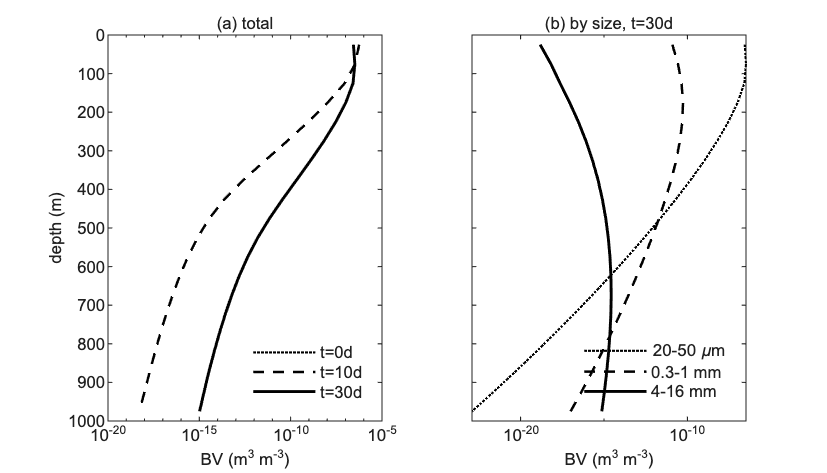
\includegraphics[width=0.85\textwidth]{../figures/example_01_profile.png}
\caption{Example~1 output. \textit{Left}: total biovolume depth profiles
at $t = 0$ (dotted), 10~days (dashed), and 30~days (solid) on a log scale.
\textit{Right}: biovolume by size group at $t = 30$~days. The largest bins
(8--16~mm) have exited the domain; intermediate bins reach 300--500~m;
small bins (20--50~$\mu$m) have settled only 30--75~m.}
\label{fig:ex01}
\end{figure}

\clearpage
% ---------------------------------------------------------------------
\section{Example 2: Depth-Varying Turbulence and Disaggregation}
\label{sec:ex02}
(in file: \texttt{scripts/examples/run\_example\_02.m})
% ---------------------------------------------------------------------

\subsection{Overview}

This experiment introduces depth-varying turbulence, operator-split
disaggregation, and an observation-based flux boundary condition.
The model is forced with daily $\varepsilon(z,t)$ profiles from EXPORTS-NA
(May 2021, North Atlantic), and the daily UVP spectrum at 100~m sets the
particle flux entering the column. The 25-day forcing cycle is repeated until
the column-mean biovolume converges.

\subsection{Configuration}

Standard EXPORTS-NA production configuration:

\begin{lstlisting}
cfg.n_sections     = 30;
cfg.sinking_law    = 'kriest_8';
cfg.ds_kernel_mode = 'sinking_law';
cfg.r_to_rg        = 1.6;
cfg.alpha          = 0.10;
cfg.enable_coag    = true;
cfg.enable_disagg  = true;
cfg.disagg_mode    = 'operator_split';
cfg.disagg_dmax_A  = 9.39e-6 * 5;
cfg.enable_zoo     = false;
cfg.enable_microbe = false;
\end{lstlisting}

Stickiness is reduced to 0.10 from the unit value in Example~1.
Disaggregation runs in operator-split mode with the Parker constant at
$5\times$ the laboratory value, which matches EXPORTS-NA size distributions.
The convergence criterion is 1\% change in column-mean biovolume per cycle:

\begin{lstlisting}
spinup_tol = 0.01;
max_cycles  = 80;
for icyc = 1:max_cycles
    phi_before = mean(sum(Y + Yfp, 2));
    % ... run one 25-day cycle ...
    phi_after = mean(sum(Y + Yfp, 2));
    if abs(phi_after - phi_before) / max(phi_before, 1e-20) < spinup_tol
        fprintf('Converged at cycle %d\n', icyc); break;
    end
end
\end{lstlisting}

\subsection{Running the experiment}

\begin{lstlisting}[numbers=none]
cd('/Users/.../1d-model-testing/scripts/examples')
run_example_02
\end{lstlisting}

Requires \texttt{keps\_for\_dave.mat} and the EXPORTS-NA UVP \texttt{.sb}
file in \texttt{data/NA/}. Runtime: 2--5 minutes.

\subsection{Expected output}

\begin{verbatim}
Converged at cycle 13
Saved example_02_profile.png
\end{verbatim}

Figure~\ref{fig:ex02} shows the quasi-steady biovolume profile.
Near-surface turbulence fragments large aggregates, while reduced turbulence
at depth allows them to grow. The result is an exponential-like attenuation
consistent with the observed Martin power-law flux profile.

\begin{figure}[h]
\centering
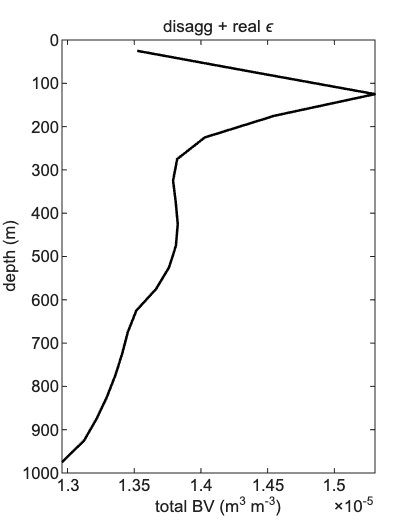
\includegraphics[width=0.42\textwidth]{../figures/example_02_profile.png}
\caption{Quasi-steady total biovolume profile for Example~2 after convergence
at spinup cycle~13. The depth- and time-varying turbulence from EXPORTS-NA and
operator-split disaggregation produce a smooth profile with exponential-like
attenuation. This profile is the baseline for adding biology in Example~3.}
\label{fig:ex02}
\end{figure}

\clearpage
% ---------------------------------------------------------------------
\section{Example 3: Full Physics with Zooplankton Grazing}
\label{sec:ex03}
(in file: \texttt{scripts/examples/run\_example\_03.m})
% ---------------------------------------------------------------------

\subsection{Overview}

Zooplankton grazing, fecal pellet production, and micro-zooplankton mining
are added to the Example~2 configuration. Filter and flux feeders
(equations~\ref{eq:filter}--\ref{eq:grazing}) follow the Stemmann et al.\
(2004) depth profiles; egested biovolume (equation~\ref{eq:fecal_prod})
enters the fecal pool \texttt{Yfp}. Aggregates and fecal pellets develop
distinct depth distributions owing to their different sinking speeds.

\subsection{Configuration}

The configuration is identical to Example~2 with the following additions:

\begin{lstlisting}
cfg.enable_zoo  = true;     % activate grazing
cfg.zoo_c       = 0.025;    % filter feeder clearance rate
cfg.zoo_s       = 1.3e-5;   % flux feeder capture cross-section
cfg.zoo_p       = 0.5;      % egestion fraction
cfg.zoo_ic      = 7;        % fecal pellets -> bin 8 (~115 um)
cfg.enable_mining = true;   % activate micro-zoo mining
\end{lstlisting}

Fecal pellets are produced into bin~8 ($d \approx 115~\mu$m,
copepod-sized) at an egestion fraction of 0.5. Mining acts on particles
above bin~12 ($d \approx 254~\mu$m).

\subsection{Running the experiment}

\begin{lstlisting}[numbers=none]
cd('/Users/.../1d-model-testing/scripts/examples')
run_example_03
\end{lstlisting}

Runtime: 3--7 minutes. Same convergence loop as Example~2.

\subsection{Expected output}

\begin{verbatim}
Converged at cycle 12
Saved example_03_profile.png
\end{verbatim}

Figure~\ref{fig:ex03} shows aggregate and fecal pellet profiles on separate
panels. Grazing steepens the aggregate attenuation relative to Example~2.
Fecal pellets ($w_\mathrm{fp} \approx 69$~m~day$^{-1}$) are concentrated
above 200~m; their rapid removal from the upper column leaves a small but
sustained contribution at depth from zooplankton distributed throughout the
column.

\begin{figure}[h]
\centering
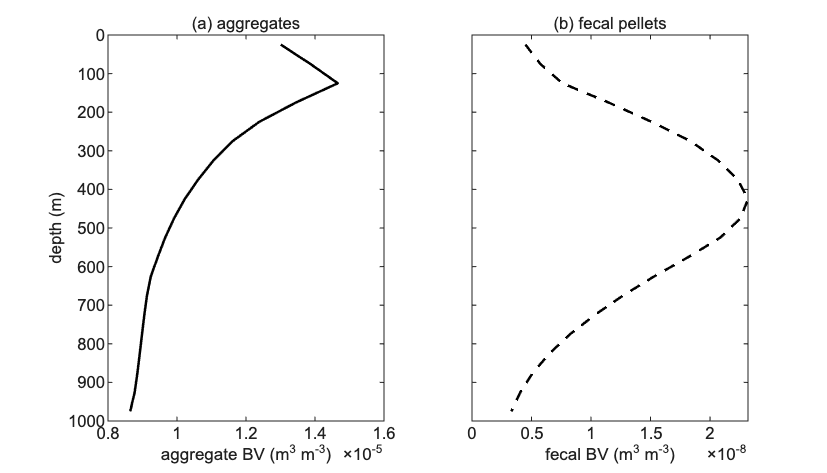
\includegraphics[width=0.82\textwidth]{../figures/example_03_profile.png}
\caption{Quasi-steady biovolume profiles for Example~3. Left: marine snow
aggregates. Right: fecal pellets. Fecal pellets are confined near the surface
because they sink $\approx$16 times faster than aggregates of the same size.
The aggregate profile shows steeper attenuation than Example~2 due to the
additional grazing sink.}
\label{fig:ex03}
\end{figure}

\clearpage
% ---------------------------------------------------------------------
\section{Example 4: Microbial Remineralization Sensitivity}
\label{sec:ex04}
(in file: \texttt{scripts/examples/run\_example\_04.m})
% ---------------------------------------------------------------------

\subsection{Overview}

Three values of the microbial remineralization rate are compared
($r_0 = 0$, $0.01$, and $0.02$~day$^{-1}$) against the Example~3 configuration.
A non-zero $r_0$ is required to reproduce the observed factor-of-four
biovolume drop between 125 and 475~m. All three runs are normalized to the
$^{234}$Th-derived POC flux at 100~m
($F_{Th} = 4.65$~mmol~m$^{-2}$~day$^{-1}$) for a clean depth comparison.

\subsection{Configuration}

The configuration is identical to Example~3, with the microbial switch
and the three $r_0$ values set in a loop:

\begin{lstlisting}
r0_vals = [0, 0.01, 0.02];   % day^-1
for k = 1:3
    cfg.enable_microbe = (r0_vals(k) > 0);
    cfg.microbe_r0     = r0_vals(k);
    % ... run and store flux profile ...
end
\end{lstlisting}

\subsection{Running the experiment}

\begin{lstlisting}[numbers=none]
cd('/Users/.../1d-model-testing/scripts/examples')
run_example_04
\end{lstlisting}

Runtime: $\approx$10--15 minutes (three spinup runs).

\subsection{Expected output}

\begin{verbatim}
r0=0.000  Converged cycle 12
r0=0.010  Converged cycle 11
r0=0.020  Converged cycle 11
Saved example_04_flux.png
\end{verbatim}

The figure shows three depth profiles of size-integrated biovolume flux
(Figure~\ref{fig:ex04}). With $r_0 = 0$, the flux is nearly flat below
300~m. With $r_0 = 0.02$~day$^{-1}$, it drops by a factor of four between
100 and 500~m, consistent with Martin-curve observations. The best-fit value
$r_0 = 0.014$~day$^{-1}$ falls between the two non-zero curves.

\begin{figure}[ht]
\centering
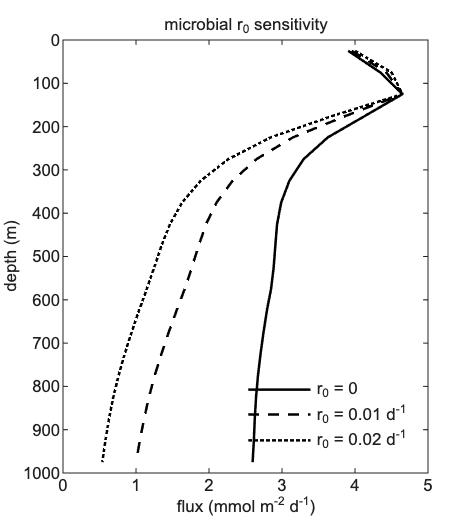
\includegraphics[width=0.45\textwidth]{../figures/example_04_flux.png}
\caption{Example~4 output. Particle flux versus depth for three
remineralization rates: $r_0 = 0$ (solid), $r_0 = 0.01$~day$^{-1}$ (dashed),
and $r_0 = 0.02$~day$^{-1}$ (dotted). All profiles are scaled to match the
$^{234}$Th flux at 100~m. Higher $r_0$ produces stronger attenuation with depth.}
\label{fig:ex04}
\end{figure}

\clearpage
% ---------------------------------------------------------------------
\section{Example 5: Full Model Comparison to EXPORTS-NA}
\label{sec:ex05}
(in file: \texttt{scripts/examples/run\_example\_05.m})
% ---------------------------------------------------------------------

\subsection{Overview}

All physics are active at the best-fit parameter values ($\alpha = 0.093$,
\texttt{bc\_scale}~$= 0.42$, $r_0 = 0.014$~day$^{-1}$;
see Section~\ref{sec:param_groups}). The quasi-steady biovolume profile is
compared to UVP observations from EXPORTS-NA at 125, 325, and 475~m.
Output includes a depth profile of total biovolume (aggregates plus fecal
pellets) and a bar chart of model/obs ratios. Good agreement is expected at
225--475~m; under-prediction at 125~m reflects the point-injection boundary
condition; over-prediction below 500~m indicates that deep loss mechanisms
(e.g., DVM redistribution) are not yet represented.

\subsection{Configuration}

All physics are on, parameters set to the best-fit values:

\begin{lstlisting}
cfg.alpha          = 0.093;
cfg.enable_microbe = true;
cfg.microbe_r0     = 0.014;
cfg.enable_mining  = true;
bc_scale           = 0.42;
phi_bc_daily       = bc.phi_bc_daily * bc_scale;
\end{lstlisting}

UVP data are filtered to 100--2000~$\mu$m; model output is averaged over
cast days at each comparison depth.

\subsection{Running the experiment}

\begin{lstlisting}[numbers=none]
cd('/Users/.../1d-model-testing/scripts/examples')
run_example_05
\end{lstlisting}

Requires the same UVP and turbulence files as Examples~2--4. Runtime:
3--5 minutes.

\subsection{Expected output}

\begin{verbatim}
Converged at cycle 13
model/obs at 125m: 0.62
model/obs at 325m: 0.90
model/obs at 475m: 0.87
Saved example_05_full_model.png
\end{verbatim}

Agreement is closest at 325 and 475~m. The under-prediction at 125~m
reflects the point-injection boundary condition rather than a distributed
surface source. The ratio bar chart quantifies the fit at each cast depth.

\begin{figure}[ht]
\centering
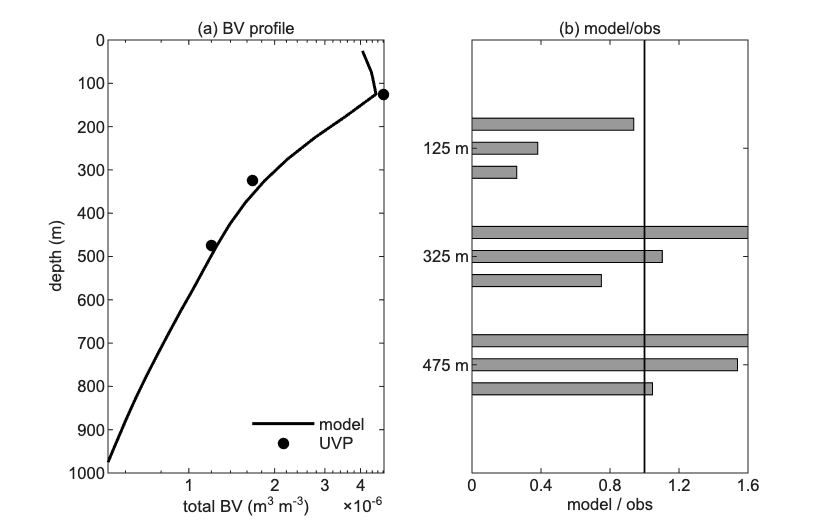
\includegraphics[width=0.82\textwidth]{../figures/example_05_full_model.png}
\caption{Example~5 output. \textit{Left}: total biovolume depth profile
(model: solid line; UVP observations: circles) on a log scale.
\textit{Right}: model/obs ratio at 125, 325, and 475~m. A ratio of~1
(vertical line) indicates exact agreement.}
\label{fig:ex05}
\end{figure}

% =====================================================================
\chapter{Common Errors and How to Fix Them}
% =====================================================================

Each entry below describes a symptom, its likely cause, and the fix.

\textit{Undefined function \textup{\texttt{ColumnGrid}} (or any \texttt{src/} class).}
The \texttt{src/} directory is not on the MATLAB path.
Check that \texttt{script\_dir = fileparts(mfilename('fullpath'))} and
\texttt{addpath(fullfile(script\_dir, '..', '..', 'src'))} both appear at
the top of the script. Run \texttt{which ColumnGrid} to confirm MATLAB can
see the file. Do not add paths globally in \texttt{startup.m}; the
per-script pattern avoids conflicts between model versions.

\textit{Negative concentrations appear during the run.}
The upwind scheme is conditionally stable: the Courant number
$\mathrm{CFL} = w_\mathrm{max}\,\Delta t / \Delta z$ must stay below~1.
With $n_\mathrm{sections} = 30$, $\Delta t = 0.25$~day, and
$\Delta z = 50$~m the CFL is approximately 0.48 ($96 \times 0.25 / 50$), which is stable.
If you increase $n_\mathrm{sections}$ (larger bins, higher sinking speeds),
reduce $\Delta t$ accordingly. Never use the Lax-Wendroff scheme
(\texttt{cfg.transport\_scheme = 'lax\_wendroff'}) in production; it
produces negative oscillations near sharp gradients.

\textit{Transfer efficiency is unrealistically high (above 10\%).}
Check \texttt{n\_sections}. With $n = 20$ the largest model bin sits at
about 6~mm and disaggregation at the base of the column is weak, so
particles pile up in the deep bins and the bottom flux is greatly
overestimated. Always use $n_\mathrm{sections} = 30$ with
$\Delta t = 0.25$~day for production runs.

\textit{The spinup loop runs all 80 cycles without converging.}
First, verify that \texttt{phi\_bc\_daily} is non-zero: run
\texttt{max(phi\_bc\_daily(:))} and confirm the result is finite and
positive. If the UVP file path is wrong, \texttt{get\_daily\_bc\_at\_depth}
silently returns zeros and the column drains completely.
Second, check that \texttt{enable\_disagg = true} and
\texttt{disagg\_dmax\_A} is set; without disaggregation the column state
drifts upward indefinitely.

\textit{Error: \textup{\texttt{operator\_split}} requires \textup{\texttt{disagg\_dmax\_cm}} or \textup{\texttt{disagg\_dmax\_A}}.}
Set \texttt{cfg.disagg\_dmax\_A = 9.39e-6 * 5} (Parker scaling with
EXPORTS calibration) or \texttt{cfg.disagg\_dmax\_cm = 1.0} for a fixed
$D_\mathrm{max}$ of 1~cm. The error is raised by
\texttt{SimulationConfig.validate()} before any time integration begins.

\textit{Unknown sinking law \textup{\texttt{'kriest8'}} (or similar).}
The accepted string is \texttt{'kriest\_8'} with an underscore. Check
\texttt{SettlingVelocityService.m} for the full list of valid names.
Common mistakes: \texttt{'Kriest8'} (wrong case), \texttt{'kriest'} (no
number), \texttt{'current'} (legacy placeholder, gives wrong sinking speeds).

\textit{Model biovolume is 2--10 times higher than UVP at all depths.}
The raw UVP data contains 85--93\% zooplankton by biovolume; the model
represents only non-zooplankton particles. Apply the 100--2000~$\mu$m
size filter (\texttt{mask\_uvp}) and set \texttt{bc\_scale = 0.42} as
described in Chapter~\ref{sec:params}. If the deep excess persists after
filtering, increase \texttt{microbe\_r0} from 0 toward 0.02~day$^{-1}$
to add microbial remineralization.

\textit{Model under-predicts biovolume at 125~m even with the right parameters.}
This is a known geometric limitation. The flux boundary condition is
injected at a single 50-m layer (layers~2, depth 75--125~m). In reality
the surface source is distributed over the mixed layer. The single-layer
injection produces a geometric deficit directly above the injection depth.
A model/obs ratio of 0.6 at 125~m is expected and does not indicate a
parameter error. A Crank-Nicolson transport scheme with a distributed BC
would reduce this artifact and is planned for a future version.

\textit{NaN values appear in \textup{\texttt{Y}} after the first time step.}
A NaN typically propagates from the kernel matrix or the turbulence
profile. Check \texttt{keps\_day} for any NaN or zero entries;
\texttt{eps = 0} produces a division-by-zero in the shear kernel.
The EXPORTS turbulence file occasionally has a missing profile on one
day; replace it with the temporal mean of the surrounding days.

% =====================================================================
\chapter*{References}
\addcontentsline{toc}{chapter}{References}
% =====================================================================

Burd, A. B., \& Jackson, G. A. (2009). Particle aggregation.
\textit{Annual Review of Marine Science}, \textit{1}, 65--90.
\href{https://doi.org/10.1146/annurev.marine.010908.163904}{https://doi.org/10.1146/annurev.marine.010908.163904}

Gelbard, F., Tambour, Y., \& Seinfeld, J. H. (1980). Sectional representations
for simulating aerosol dynamics. \textit{Journal of Colloid and Interface Science},
\textit{76}(2), 541--556.
\href{https://doi.org/10.1016/0021-9797(80)90394-X}{https://doi.org/10.1016/0021-9797(80)90394-X}

Iversen, M. H., \& Ploug, H. (2013). Temperature effects on carbon-specific
respiration rate and sinking velocity of diatom aggregates.
\textit{Biogeosciences}, \textit{10}, 4073--4085.
\href{https://doi.org/10.5194/bg-10-4073-2013}{https://doi.org/10.5194/bg-10-4073-2013}

Jackson, G. A. (1990). A model of the formation of marine algal flocs by physical
coagulation processes. \textit{Deep-Sea Research}, \textit{37}(8), 1197--1211.
\href{https://doi.org/10.1016/0198-0149(90)90038-W}{https://doi.org/10.1016/0198-0149(90)90038-W}

Jackson, G. A., \& Burd, A. B. (1998). Aggregation in the marine environment.
\textit{Environmental Science \& Technology}, \textit{32}(19), 2805--2814.
\href{https://doi.org/10.1021/es9708292}{https://doi.org/10.1021/es9708292}

Kriest, I. (2002). Different parameterizations of marine snow in a 1D-model
and their influence on the carbon flux distribution.
\textit{Deep-Sea Research I}, \textit{49}, 2133--2162.
\href{https://doi.org/10.1016/S0967-0637(02)00095-7}{https://doi.org/10.1016/S0967-0637(02)00095-7}

Li, X., \& Logan, B. E. (1995). Size distributions and fractal properties of
particles during a simulated phytoplankton bloom in a mesocosm.
\textit{Deep-Sea Research II}, \textit{42}(1), 125--145.
\href{https://doi.org/10.1016/0967-0645(95)00007-Q}{https://doi.org/10.1016/0967-0645(95)00007-Q}

Li, X., \& Logan, B. E. (1997). Collision frequencies of fractal aggregates with
small particles by differential sedimentation and laminar shear flow.
\textit{Environmental Science \& Technology}, \textit{31}(4), 1229--1236.
\href{https://doi.org/10.1021/es960672b}{https://doi.org/10.1021/es960672b}

Logan, B. E., \& Wilkinson, D. B. (1990). Fractal geometry of marine snow and
other biological aggregates. \textit{Limnology and Oceanography}, \textit{35}(1),
130--136.
\href{https://doi.org/10.4319/lo.1990.35.1.0130}{https://doi.org/10.4319/lo.1990.35.1.0130}

Millero, F. J., \& Poisson, A. (1981). International one-atmosphere equation of
state of seawater. \textit{Deep-Sea Research A}, \textit{28}(6), 625--629.
\href{https://doi.org/10.1016/0198-0149(81)90122-9}{https://doi.org/10.1016/0198-0149(81)90122-9}

Parker, D. S., Kaufman, W. J., \& Jenkins, D. (1972). Floc breakup in turbulent
flocculation processes. \textit{Journal of the Sanitary Engineering Division, ASCE},
\textit{98}, 79--99.

Ploug, H., Iversen, M. H., \& Fischer, G. (2008). Ballast, sinking velocity, and
apparent diffusivity within marine snow and zooplankton fecal pellets.
\textit{Limnology and Oceanography}, \textit{53}(5), 1878--1886.
\href{https://doi.org/10.4319/lo.2008.53.5.1878}{https://doi.org/10.4319/lo.2008.53.5.1878}

Sharqawy, M. H., Lienhard, J. H., \& Zubair, S. M. (2010). Thermophysical
properties of seawater: a review of existing correlations and data.
\textit{Desalination and Water Treatment}, \textit{16}(1--3), 354--380.
\href{https://doi.org/10.5004/dwt.2010.1079}{https://doi.org/10.5004/dwt.2010.1079}

Smoluchowski, M. (1917). Versuch einer mathematischen Theorie der
Koagulationskinetik kolloider L\"{o}sungen. \textit{Zeitschrift f\"{u}r Physikalische
Chemie}, \textit{92}, 129--168.

Stemmann, L., Jackson, G. A., \& Ianson, D. (2004a). A vertical model of particle
size distributions and fluxes in the midwater column that includes biological
and physical processes, Part~I. \textit{Deep-Sea Research I}, \textit{51}, 865--884.
\href{https://doi.org/10.1016/j.dsr.2004.01.002}{https://doi.org/10.1016/j.dsr.2004.01.002}

Stemmann, L., Jackson, G. A., \& Gorsky, G. (2004b). A vertical model of particle
size distributions and fluxes in the midwater column that includes biological
and physical processes, Part~II. \textit{Deep-Sea Research I}, \textit{51}, 885--908.
\href{https://doi.org/10.1016/j.dsr.2004.01.003}{https://doi.org/10.1016/j.dsr.2004.01.003}

Tarantola, A., \& Valette, B. (1982). Generalized nonlinear inverse problems
solved using the least squares criterion.
\textit{Reviews of Geophysics and Space Physics}, \textit{20}(2), 219--232.
\href{https://doi.org/10.1029/RG020i002p00219}{https://doi.org/10.1029/RG020i002p00219}

Turner, J. T. (2002). Zooplankton fecal pellets, marine snow and sinking
phytoplankton blooms. \textit{Aquatic Microbial Ecology}, \textit{27}, 57--102.
\href{https://doi.org/10.3354/ame027057}{https://doi.org/10.3354/ame027057}

\end{document}
